\documentclass{article}
\usepackage{amsmath}
\usepackage[utf8]{inputenc}
\usepackage[T1]{fontenc}
\usepackage[ngerman]{babel}
\usepackage[shortlabels]{enumitem}
\usepackage{amsfonts}
\usepackage[left=3cm,right=2cm,top=2.5cm,bottom=2cm]{geometry}
\usepackage{amssymb}
\usepackage{cancel}
\usepackage{karnaugh-map}
\usepackage{xcolor}
\usepackage{caption}
\usepackage{subcaption}

\newcommand{\nyet}{\overline}

\title{Formale Grundlagen: Übung 4}
\author{Alexander Waldenmaier, Tutorin: Constanze Merkt}

\begin{document}
    \maketitle

    \subsection*{Aufgabe 4.1}
    Es gibt insgesamt $2^n+1$ numerisch monotone Boolesche Funktionen $f:\mathcal{B}^n \rightarrow \mathcal{B}$. \\\\
    Begründung: Im einfachsten Fall, $n=1$ gibt es exakt 3 monotone Funktionen: $f_1(x) = 0, f_2(x) = x, f_3(x) = 1$. Die Funktion $f_4(x) = \overline{x}$ erfüllt die Bedingung nicht, da $f_4(x)=1 \nleq 0=f_4(y)$ mit $x=0<1=y$. Aus einer Wertetabelle kann man leicht das Verhalten für höhere $n$ ablesen: 
    \begin{table}[h]
        \centering
        \begin{tabular}{c|cccc||cccc}
            $(x_1, x_2, \ldots, x_n)_{10}$ & $x_1$ & $x_2$ & $\cdots$ & $x_n$ & $f_1$ & $f_2$ & $\cdots$ & $f_{2n+1}$\\ \hline
            0 & 0 & 0 & $\cdots$ & 0 & 0 & 0 & $\cdots$ & 1 \\
            1 & 0 & 0 & $\cdots$ & 1 & 0 & 0 & $\cdots$ & 1 \\
            $\vdots$ & $\vdots$ & $\vdots$ & $\vdots$ & $\vdots$ & $\vdots$ & $\vdots$ & $\vdots$ & $\vdots$ \\
            $2n-1$ & 1 & 1 & $\cdots$ & 1 & 0 & 1 & $\cdots$ & 1 \\
        \end{tabular}
    \end{table}\\
    Betrachtet man die möglichen Funktionen $f_i$ in der Tabelle rechts, so erkennt man, dass für größer werdende $i$ die "`Grenze"', bei der die Funktion nicht mehr 0 sondern 1 herausgibt, sich je um eins nach oben verschiebt, bis irgendwann für jeden beliebigen Input $x$ der Funktionswert stets 1 ergibt. 


    \subsection*{Aufgabe 4.2}
    Zunächst muss $f$ in Ringsummennormalform (RSNF) umgewandelt werden, da darin nur $\oplus$ und $\land$ enthalten sind. Wir nutzen ein KV-Diagramm um eine orthogonale Form von $f$ herzustellen:\\
    \begin{minipage}[t]{0.67\textwidth}
        \begin{align*}
            f(x, y, z) &= (x \nyet{z}) \lor (x \nyet{y}) \lor (\nyet{x} y z) \\
            &\stackrel{\text{KV}}{=} x \nyet{y} \nyet{z} \lor x \nyet{y} z \lor x y \nyet{z} \lor \nyet{x} y z \\
            &=x \nyet{y} \nyet{z} \oplus x \nyet{y} z \oplus x y \nyet{z} \oplus \nyet{x} y z \\
            &=x (y \oplus 1) (z \oplus 1) \oplus x (y \oplus 1) z \oplus x y (z \oplus 1) \oplus (x \oplus 1) y z \\
            &=\cancel{xyz} \oplus \cancel{xy} \oplus \cancel{xz} \oplus x \oplus \cancel{xyz} \oplus \cancel{xz} \oplus \cancel{xyz} \oplus \cancel{xy} \oplus \cancel{xyz} \oplus yz \\
            &= x \oplus yz
        \end{align*}
    \end{minipage}
    \begin{minipage}[t]{0.4\textwidth}
        \hfill\\\\
        \begin{karnaugh-map}[4][2][1][$z, x$][$y$]
            \manualterms{0,1,0,1,0,1,1,0}
        \end{karnaugh-map}    
    \end{minipage} \\
    Damit lässt sich die folgende Schaltung implementieren:\\\\
    \begin{figure}[h]
        \centering
        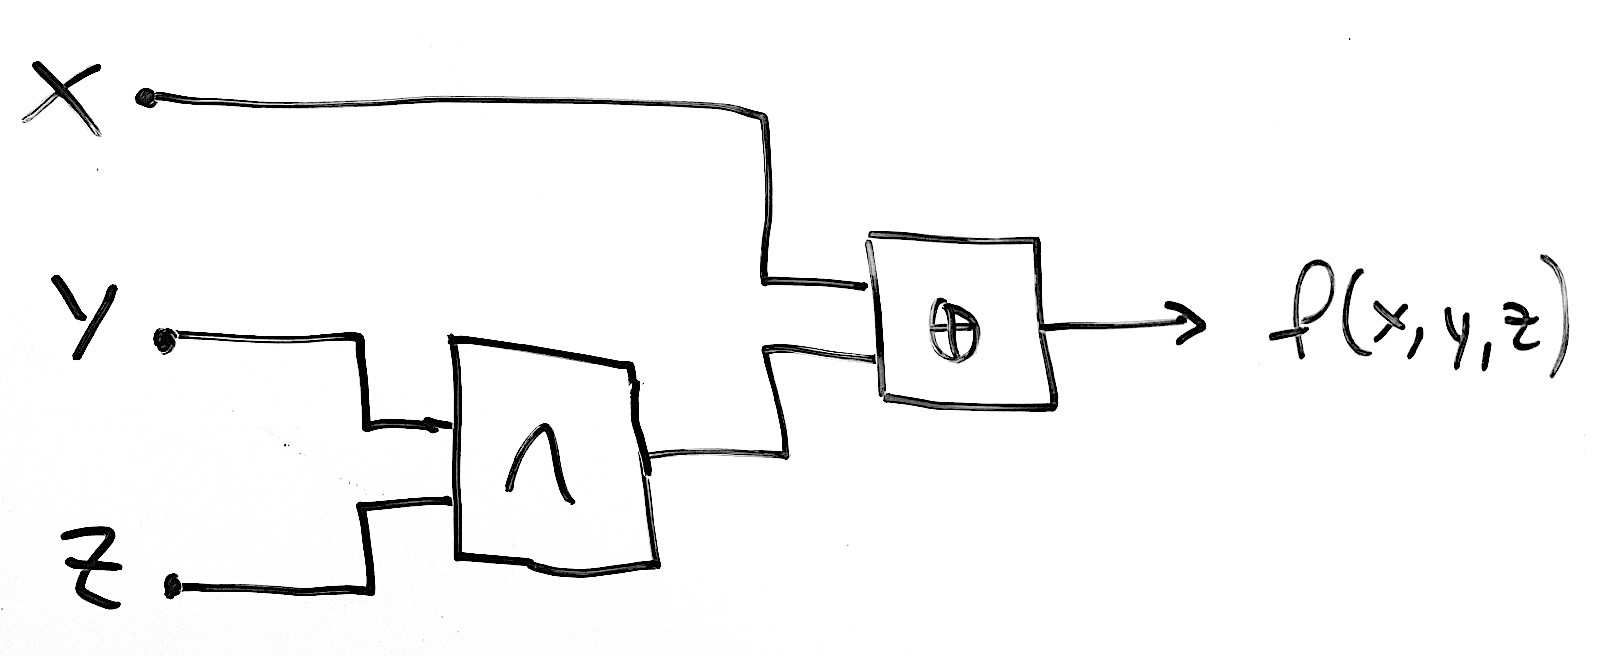
\includegraphics[width=0.4\textwidth]{schaltung1.jpeg}
    \end{figure}
    


    \subsection*{Aufgabe 4.3}
    Wir betrachten zunächst die folgende einfache Multiplikation zweier Binärzahlen:
    \begin{table}[h]
        \centering
        \begin{tabular}{crl}
            & $1011 \cdot \textcolor{green}{1}\textcolor{red}{0}\textcolor{green}{1}\textcolor{red}{0}$ & = \\ \hline
            & $\textcolor{green}{1011000}$ \\
           +& $\textcolor{red}{0000000}$ \\
           +& $\textcolor{green}{0010110}$ \\
           +& $\textcolor{red}{0000000}$ \\ 
           c& $\textcolor{gray}{0100000}$ \\ \hline
           s& 1101110
       \end{tabular} 
    \end{table}

    Die rechte Zahl hat eine 1 an der 1. und der 3. Stelle (0-basiert). Demnach wird die linke Zahl einmal um 3 Bits nach links verschoben (rechts mit Nullen aufgefüllt) bzw. einmal um 1 Bit nach links verschoben. Beide resultierenden Zahlen (grün markiert) werden dann addiert, um das Ergebnis der Multiplikation zu erhalten. Für jede 0 in der rechten Zahl muss nichts addiert werden (rot markiert).

    Generell lässt sich also sagen. Das Ergebis der Multiplikation, $m$, wird zunächst mit 0 initialisiert. Dann werden alle Stellen $b_i$ von $b$ vom LSB bis hin zum MSB durchgegangen. Mit jeder Erhöhung von $i$ wird die Zahl $a$ um ein Bit nach links verschoben und rechts mit einer Null ergänzt. An jeder Stelle $i$, an der $b_i = 1$ ist, wird die derzeitige (verschobene) Version von $a$ zu $m$ hinzuaddiert (ansonsten wird 0 addiert). Sobald alle Stellen von $b$ durchgegangen sind, ist die Multiplikation beendet und das Ergebnis $m$ kann ausgelesen werden. 

    Um zwei $n$-stellige Binärzahlen $a$ und $b$ zu addieren, benötigt es $n$ miteinander verschaltetete Volladdierer (siehe Abbildung \ref{f:naddierer}). Dabei bekommt der Volladdierer (VA), der die beiden Least Significant Bits (LSB) addiert, einen "`Carry-In"' von 0 und gibt seinen "`Carry-Out"' an den darauffolgenden VA weiter. Diese Kette führt sich fort, bis am Ende alle Stellen $s_i$ der Summe $s$ bekannt sind, sowie ein optionaler Carry-Out aus dem letzten VA. Dies würde gleichzeitig einen Overflow signalisieren. Die Größe eines Volladdierers (wie im Skript) beträgt $C(\text{add}) = 5$, die Tiefe $D(\text{add}) = 3$. Für den $n$-stelligen Volladdierer gilt: $C(\text{nadd}) = n\cdot C(\text{add}) = 5n$, $D(\text{nadd}) = n \cdot D(\text{add}) = 3n$ (da jeder VA zunächst auf den Carry-In vom vorigen VA warten muss).
    \begin{figure}[h]
        \centering
        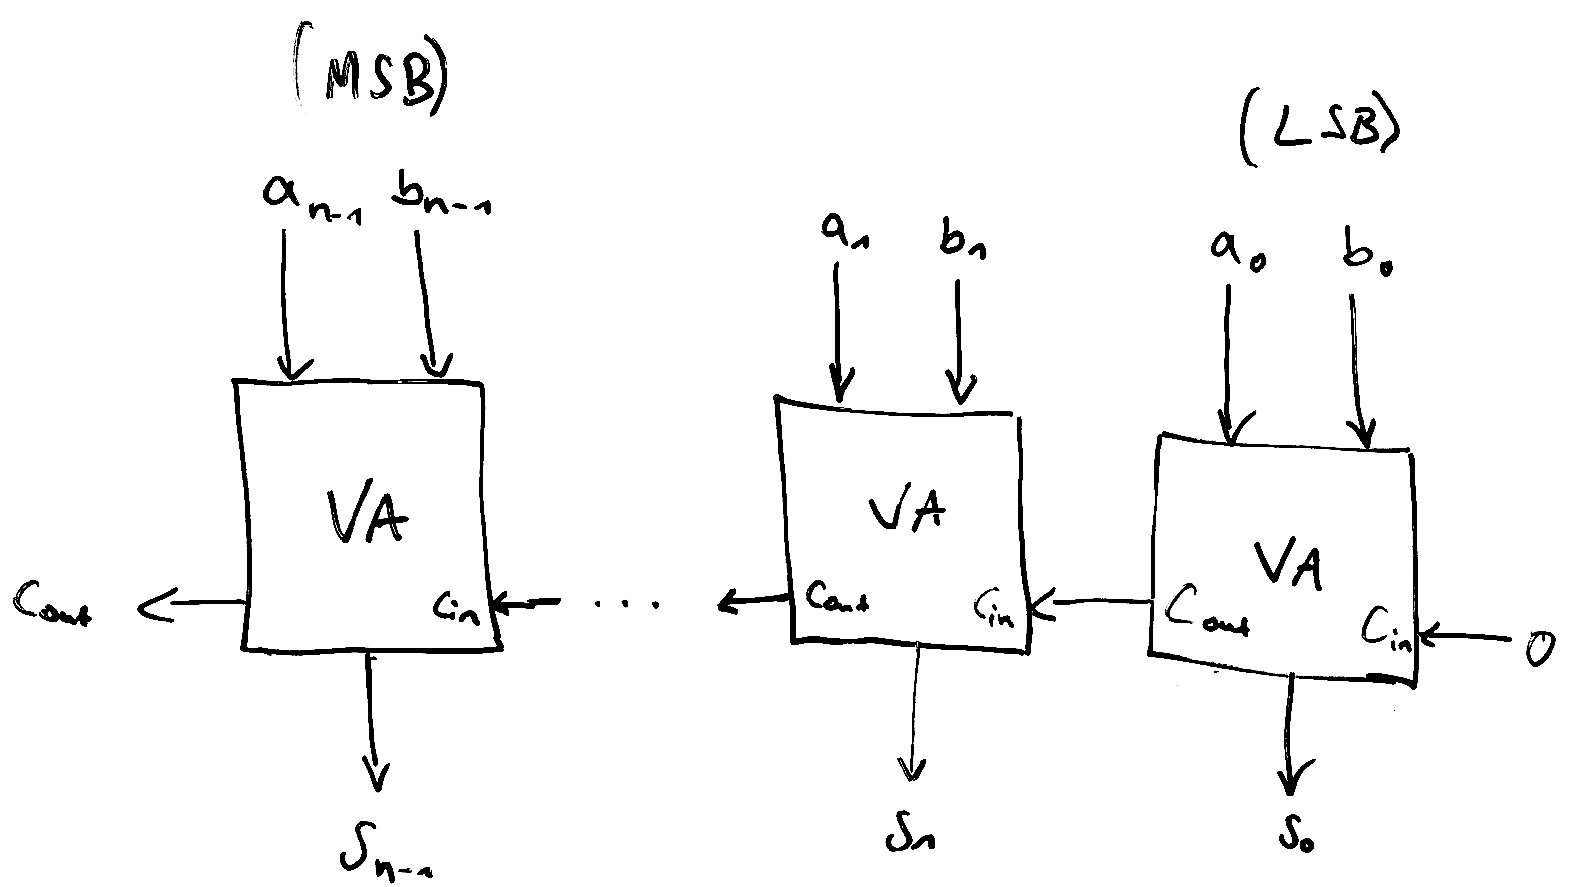
\includegraphics[width=0.6\textwidth]{naddierer.jpeg}
        \caption{$n$-stelliger Volladdierer (NVA)}
        \label{f:naddierer}
    \end{figure}

    Um den Multiplikator in einer Schaltung umzusetzen, wird zusätzlich noch ein Multiplexer "`selector"' benötigt. Abhängig von einer Variable $x$ (in diesem Fall $b_i$) wird entweder $a$ oder $b$ ausgewählt (in diesem Fall $a_j$ oder 0). Ein solcher Selektor ist in Abbildung \ref{f:sel} dargestellt. Seine Größe beträgt $C(\text{sel}) = 3$ und seine Tiefe $D(\text{sel}) = 2$. Die $n$-stellige Variante verbindet $n$ solcher Selektoren und ist in Abbildung \ref{f:nsel} dargestellt. Die Größe beträgt $C(\text{nsel}) = n \cdot C(\text{sel}) = 3n$ und die Tiefe $D(\text{nsel}) = 2$. 

    \begin{figure}[h]
        \begin{subfigure}[b]{0.5\textwidth}
            \centering
            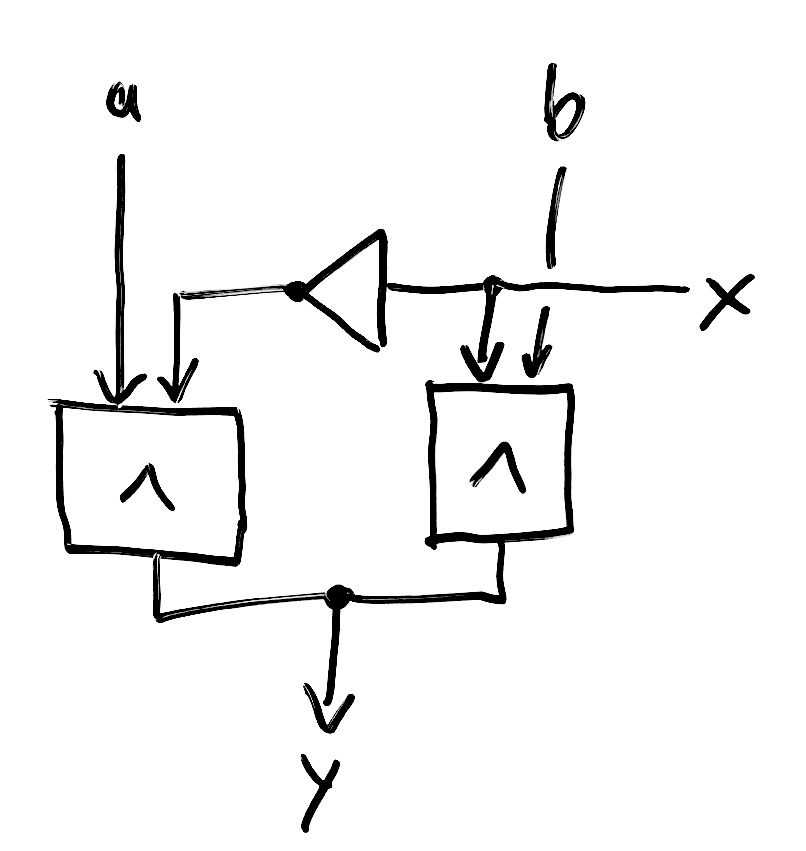
\includegraphics[width=0.5\textwidth]{sel.jpeg}
            \caption{1-stelliger Selektor (sel)}
            \label{f:sel}
        \end{subfigure}
        \begin{subfigure}[b]{0.5\textwidth}
            \centering
            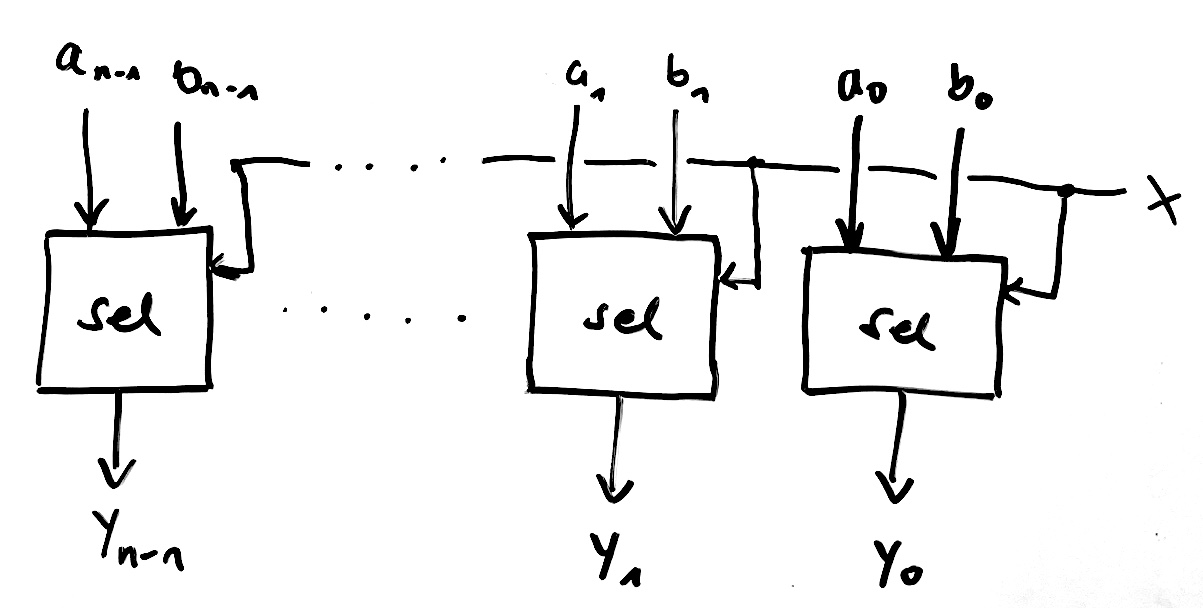
\includegraphics[width=\textwidth]{nsel.jpeg}
            \caption{$n$-stelliger Selektor (n-sel)}
            \label{f:nsel}
        \end{subfigure}
        \caption{Multiplexer}
        \label{f:multiplexer}
    \end{figure}

    Mit den $n$-stelligen Volladdierern und Multiplexern lässt sich nun der Multiplikator zusammenbauen, der in Abbildung \ref{f:multiplikator} dargestellt ist. Das Ergebnis der Multiplikation zum $i$-ten Schritt steckt jeweils in der Variable $m^{(i)}$, die der Reihe nach an die $n$ $n$-stelligen Volladdierer (NVA) übergeben wird. Diese erhalten als zweiten Summanden die um $i$ Bits verschobene Zahl $a$, oder 0 (wenn $b_i$ 0 war). Es ist eine Menge an Verdrahtung notwendig, um die Zahl $n$ Bits der Zahl $a$ "`aufzudröseln"' und an die $n$ Selektoren zu übergeben. Die Größe des Multiplikators beträgt $C(\text{nmult}) = n\cdot(C(\text{nsel}) + C(\text{nadd})) = n \cdot (5n + 3n) = 8n^2$ und die Tiefe $D(\text{nmult}) = n\cdot D(\text{nadd}) + D(\text{nsel}) = 3n^2 + 2$ (da der letzte Volladdierer zunächst auf das Ergebnis aller vorigen NVA warten muss).
    \begin{figure}[h]
        \centering
        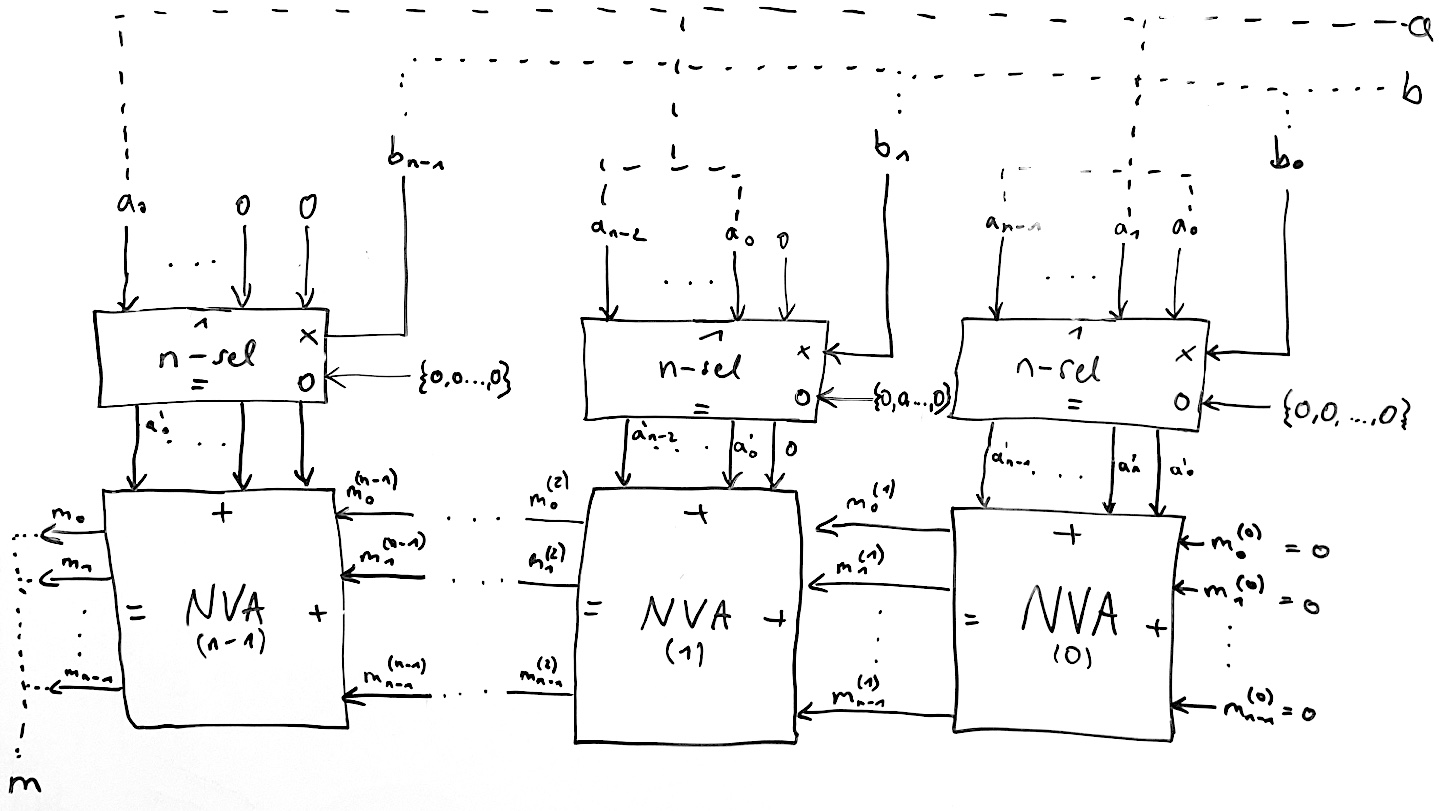
\includegraphics[width=0.9\textwidth]{multiplikator.jpeg}
        \caption{$n$-stelliger Multiplikator}
        \label{f:multiplikator}
    \end{figure}

    \subsection*{Aufgabe 4.4}
    \begin{enumerate}
        \item[a)]
        \begin{align*}
            f(x,y,z) &= () + () \\
            &= () \cdot () + () \cdot () \\
            &= \nyet{()} \cdot () + () \cdot \nyet{()} \\
            &= \nyet{z} \cdot (() + ()) + z \cdot \nyet{(() + ())} \\
            &= \nyet{z} \cdot (()\cdot () + ()\cdot ()) + z \cdot \nyet{()\cdot () + ()\cdot ()} \\
            &= \nyet{z} \cdot (\nyet{()}\cdot x + y\cdot \nyet{()}) + z \cdot \nyet{\nyet{()}\cdot x + y\cdot \nyet{()}} \\
            &= \nyet{z} \cdot (\nyet{y} x + y \nyet{x}) + z \cdot \nyet{\nyet{y} x + y \nyet{x}} \\
        \end{align*}
        \textit{Die leeren Klammern stellen jeweils einen Platzhalter für weiterfolgende Teile der Schaltung dar.}
        \item[b)]
        \begin{itemize}
            \item Größe: 4x NOT, 4x AND, 2x OR $\Rightarrow C(S) = 10$
            \item Tiefe (Längster Pfad): x $\rightarrow$ NOT $\rightarrow$ AND $\rightarrow$ OR $\rightarrow$ NOT $\rightarrow$ AND $\rightarrow$ OR $\Rightarrow D(S)=6$
        \end{itemize}
    \end{enumerate}
\end{document}